\documentclass[]{article}
\usepackage[T1]{fontenc}
\usepackage{lmodern}
\usepackage{amssymb,amsmath}
\usepackage{ifxetex,ifluatex}
\usepackage{graphicx}

\usepackage{fixltx2e} % provides \textsubscript
% use microtype if available
\IfFileExists{microtype.sty}{\usepackage{microtype}}{}
\ifnum 0\ifxetex 1\fi\ifluatex 1\fi=0 % if pdftex
  \usepackage[utf8]{inputenc}
\else % if luatex or xelatex
  \usepackage{fontspec}
  \ifxetex
    \usepackage{xltxtra,xunicode}
  \fi
  \defaultfontfeatures{Mapping=tex-text,Scale=MatchLowercase}
  \newcommand{\euro}{€}
\fi
% Redefine labelwidth for lists; otherwise, the enumerate package will cause
% markers to extend beyond the left margin.
\makeatletter\AtBeginDocument{%
  \renewcommand{\@listi}
    {\setlength{\labelwidth}{4em}}
}\makeatother
\usepackage{enumerate}
\usepackage{graphicx}
% We will generate all images so they have a width \maxwidth. This means
% that they will get their normal width if they fit onto the page, but
% are scaled down if they would overflow the margins.
\makeatletter
\def\maxwidth{\ifdim\Gin@nat@width>\linewidth\linewidth
\else\Gin@nat@width\fi}
\makeatother
\let\Oldincludegraphics\includegraphics
\renewcommand{\includegraphics}[1]{\Oldincludegraphics[width=\maxwidth]{#1}}
\ifxetex
  \usepackage[setpagesize=false, % page size defined by xetex
              unicode=false, % unicode breaks when used with xetex
              xetex]{hyperref}
\else
  \usepackage[unicode=true]{hyperref}
\fi
\hypersetup{breaklinks=true,
            bookmarks=true,
            pdfauthor={},
            pdftitle={},
            colorlinks=true,
            urlcolor=blue,
            linkcolor=magenta,
            pdfborder={0 0 0}}
\setlength{\parindent}{0pt}
\setlength{\parskip}{6pt plus 2pt minus 1pt}
\setlength{\emergencystretch}{3em}  % prevent overfull lines
\setcounter{secnumdepth}{0}

\author{}
\date{}

\begin{document}

\section{Bios 301: Assignment 4}

\emph{Due Friday, 6 December, 12:00 PM}

50 points total.

Submit a single knitr (either \texttt{.rnw} or \texttt{.rmd}) file,
along with a valid PDF (or html) output file. Inside the file, clearly
indicate which parts of your responses go with which problems (you may
use the original homework document as a template). Raw R code/output or
word processor files are not acceptable.

\subsubsection{Question 1}

10 points

Use the simulated results from question 3 in assignment 3 to
\emph{exactly} reproduce the following plot in ggplot2. Please show your
code.:

\begin{figure}[htbp]
\centering
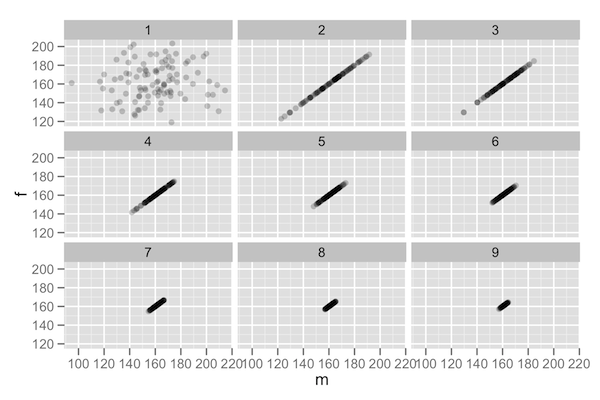
\includegraphics{a4q1.png}
\caption{generations plot}
\end{figure}

\subsubsection{Question 2}

6 points

Approximate the probability that the proportion of heads obtained will
be between 0.50 and 0.52 when a fair coin is tossed

\begin{enumerate}[1.]
\item
  50 times.
\item
  500 times.
\end{enumerate}

\subsubsection{Question 3}

10 points

We know that the \emph{U(−1,1)} random variable has mean 0. Use a sample
of size 100 to estimate the mean and give a 95\% confidence interval.
Does the confidence interval contain 0? Repeat the above a large number
of times (say, 1000). What percentage of time does the confidence
interval contain 0? Write your code so that it produces output similar
to the following:

\begin{verbatim}
Number of trials: 10

Sample mean  lower bound  upper bound  contains mean
    -0.0733      -0.1888       0.0422             1
    -0.0267      -0.1335       0.0801             1
    -0.0063      -0.1143       0.1017             1
    -0.0820      -0.1869       0.0230             1
    -0.0354      -0.1478       0.0771             1
    -0.0751      -0.1863       0.0362             1
    -0.0742      -0.1923       0.0440             1
     0.0071      -0.1011       0.1153             1
     0.0772      -0.0322       0.1867             1
    -0.0243      -0.1370       0.0885             1

100 percent of CI's contained the mean
\end{verbatim}

\subsubsection{Question 4}

24 points

Programming with classes:

\begin{enumerate}[1.]
\item
  Create an S3 class \texttt{medicalRecord} for objects that are a list
  with the named elements \texttt{name}, \texttt{gender},
  \texttt{date\_of\_birth}, \texttt{date\_of\_admission},
  \texttt{pulse}, \texttt{temperature}, \texttt{fluid\_intake}. Note
  that an individual patient may have multiple measurements for some
  measurements (Hint: you may need to use a vector or data frame
  somewhere).
\item
  Write a \texttt{medicalRecord} method for the generic function
  \texttt{mean}, which returns averages for pulse, temperature and
  fluids. Also write a \texttt{medicalRecord} method either for
  \texttt{print}, which employs some nice formatting, perhaps arranging
  measurements by date, or \texttt{plot} that generates a composite plot
  of measurements over time.
\item
  Create a further class for a cohort (group) of patients, and write
  methods for \texttt{mean} and \texttt{print} which, when applied to a
  cohort, apply mean or print to each patient contained in the cohort.
  Hint: think of this as a ``container'' for patients.
\end{enumerate}

\end{document}
